\scanpage{18}
\mspage{9}
\uline{Definition of $\alpha$}\qquad We are going to define
\[
\alpha(\unsure{\mathcal E|\Sigma},\mathcal G,\pi,\mathfrak Z\mathord{\begin{tikzpicture}[x=1ex,y=1ex,baseline=0pt]
\fill (0.10,0.23) circle (0.08);
\draw[line width=0.45pt,line cap=round] (0.39,0.18)--(0.71,0.18);
\end{tikzpicture}})=(\Pi,\widetilde\Pi,p,\mathcal G,a)
\]
\[
\left\{\begin{array}{l}
\operatorname{Ob}\Pi=\mathfrak Z/\pi\unsure{.}\quad(\text{say }J)\\
\operatorname{Isom}(j,j')=\operatorname{Isom}_{\pi}(\mathfrak Z_j,\mathfrak Z_{j'})\\
\text{composition of arrows obvious}
\end{array}\right.\qquad\bigg|\quad\text{whence groupoid }\Pi
\]
\[
\deleted{\widetilde\Pi_j=\mathfrak Z_j}\qquad\operatorname{Ob}\widetilde\Pi=\mathfrak Z
\]
\diagram{\begin{tikzcd}[ampersand replacement=\&]
\operatorname{Isom}(z,z')=\{\mathrm{pt}\}\arrow[d]\&\begin{gathered}\forall z,z'\in\mathfrak Z\\(\widetilde\Pi\text{ discrete category}\mathord{\begin{tikzpicture}[x=1ex,y=1ex,baseline=0pt]
\fill (0.10,0.23) circle (0.08);
\draw[line width=0.45pt,line cap=round] (0.39,0.18)--(0.71,0.18);
\end{tikzpicture}})\end{gathered}\\
\operatorname{Isom}(j,j')\simeq\operatorname{Isom}(\mathfrak Z_j,\mathfrak Z_{j'})\&
\end{tikzcd}}
\deleted{(\unsure{where} $j,j'$ \unsure{the} \unsure{images}\unsure{)}}\inserted{(if $j=\dot z$, $j'=\dot z'$)}
\margin{\figure{\begin{tikzpicture}[x=1cm,y=1cm]
\draw (0,0.20)--(0,-2.40);
\node[anchor=west,inner sep=0pt] at (0.15,0) {$\widetilde\Pi$ \uline{discrete} category};
\node[anchor=west,inner sep=0pt] at (0.15,-0.38) {over $\Pi$ defined by};
\node[anchor=west,inner sep=0pt] at (0.15,-0.86) {functor};
\node[anchor=west,inner sep=0pt] at (0.95,-0.60) {\inserted{\unsure{contravariant}}};
\draw[thin] (0.94,-0.64) .. controls (0.75,-0.66) and (0.57,-0.74) .. (0.45,-0.83);
\node[inner sep=0pt] at (0,-1.35) {$\Longleftarrow$};
\node[anchor=west,inner sep=0pt] at (0.15,-1.45) {\begin{tikzcd}[ampersand replacement=\&,column sep=small]
F:\Pi^\circ\arrow[r]\&\operatorname{Ens}
\end{tikzcd}};
\node[anchor=west,inner sep=0pt] at (0.15,-2.10) {$F(j)=\mathfrak Z_j,\ldots$};
\node[anchor=west,inner sep=0pt] at (0.15,-2.72) {$\widetilde\Pi\simeq\Pi_{/F}$};
\end{tikzpicture}}}
$\downarrow$ transforms the unique \unsure{point|point} of $\operatorname{Isom}(z,z')$ into the unique 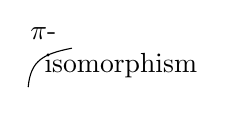
\begin{tikzpicture}[baseline=(iso.base),x=1cm,y=1cm]
\node[anchor=base west,inner sep=0pt] (iso) at (0,0) {isomorphism};
\node[anchor=base west,inner sep=0pt] at (-0.18,0.42) {\inserted{$\pi$-}};
\draw[thin,line cap=round] (-0.20,-0.18) .. controls (-0.17,0.16) and (0.00,0.24) .. (0.35,0.31);
\end{tikzpicture} $\mathfrak Z_j\mathbin{-}\mathfrak Z_{j'}$ transforming $z$ into $z'\ldots.$

For the moment we have not used $\unsure{\mathcal E|\Sigma}$ and the action of $\unsure{\mathcal E|\Sigma}$ on $\mathfrak Z$. We are going to use it now to make $\mathcal G=\unsure{\mathcal E|\Sigma}/\pi$ act on $\Pi$, and $\unsure{\mathcal E|\Sigma}$ on $\widetilde\Pi$, in a compatible way.
As $\unsure{\mathcal E|\Sigma}$ acts on $\mathfrak Z=\operatorname{Ens}(\widetilde\Pi)$, it in fact acts on $\widetilde\Pi$, associated discrete category, \deleted{\unsure{acting freely}} and \deleted{the} $\pi$ acts by $\Pi$-auto---, whence the action of $\mathcal G$ on $\pi$ by passage to the quotient.
\mspage{17}
